\cotefile{86}
\scanpage{2}

\begin{flushright}
Polyèdres réguliers\\
I
\end{flushright}

% archive sheet number: 1

\scanpage{3}

\uline{Polyèdres combinatoires}

\diagram{$\left.\begin{array}{ccccc} S&&A&&F\\ &R&&R'&\end{array}\right|\ \uline{\text{finis}}$}

\diagram{\begin{tikzcd}[ampersand replacement=\&,row sep=small,column sep=small]
R\subset S\times A\arrow[dr,dash]\&{}\&R'\subset A\times F\arrow[dl,dash]\\
\&\text{\textquotedblleft relations d'incidences\textquotedblright}\&
\end{tikzcd}}

\[
\Rightarrow\ \Phi\ \deleted{=}\ S\amalg A\amalg F
\quad\text{ens. ordonné}
\]

\[
 R''\subset S\times F,\quad
 \underset{\substack{\Vert\\R\circ R'}}{R''}=R\times_A R'
\]

\margin{\deleted{\unsure{poly}} ``géométrie d'incidences'' de dim 2}
% margin note written sideways

1) $\forall\,a\in A,\ \operatorname{card}R(a)=\operatorname{card}F(a)=2$

2) $\forall\,s\in S,\ f\in F$ avec $s<f$,

\[
 \operatorname{card}(\{a\in A\mid s<a<f)=2
\]

3) $\forall\, f\in F$, l'ens ordonné $\Phi_{<f}=\{x\in\Phi\mid x<f\}$ (qui est un \unsure{ordon|ordun|contour}) est \uline{connexe} \inserted{$\ne\varnothing$} i.e. est un polygone combinatoire (à $q(f)$ $\geq 2$ côtés)

3$'$) $\forall s\in S$, l'ens ordonné $\Phi_{>s}=\{x\in\Phi\mid x>s\}$ (``\quad '') est connexe $\ne\varnothing$ i.e., est un polygone combinatoire (à pfs $\geq 2$ côtés)

\margin{\deleted{\unsure{on exige}} \unsure{sup$^{t}$} ``polyèdre combinatoire''}
% slanted

4) Dans $\Phi$ les sup majorés existent ($\Longleftrightarrow$ les inf minorés existent)

\inserted{i.e. $x,y\in\Phi,\ \substack{x\nleq y\\ y\nleq x}\mid x,y<f\in F\Rightarrow\operatorname{Sup}(x,y)$ existe}

i.e. $\left\{\begin{aligned}
 &\text{a) Toute arête $a$ est déterminée par l'ens $\{s,s'\}$ de ses extrémités, et tte}\\
 &\text{face qui majore celles-ci majore l'arête.}\\
 &\text{b) Toute face $f$ est connue quand on connait une arête $a$ de $f$ et}\\
 &\text{un sommet de $f$ non incident, et si on connait deux}\\
 &\text{sommets de $f$ non incidents à une même arête.}
\end{aligned}\right.$

\uline{NB} Indépendamment de \uline{4)}, si $s,s'\in S,\ s\ne s',\ s,s'<a\in A$, \deleted{\unsure{alors|alors si}}

1°) $\operatorname{Sup}(s,s')$ existe sss $a=\operatorname{Sup}(s,s')$ -- \deleted{il \inserted{suff.} \unsure{faut} \inserted{sss} que $\operatorname{Sup}(s,s')$ existe, il f. et s. que} a) \deleted{On} soit seule arête qui soit incidente à $s,s'$

b) Toute face incidente à la fois à $s,s'$ l'est à $a$).

\deleted{2°) $\operatorname{Sup}(s,s')$ existe \unsure{sss}}

2°) Si $s,s'\in S,\ s,s'<f\in F$, \deleted{$s\ne s'$}, non incidents à une \deleted{\unsure{seule|même}} arête, alors $\operatorname{Sup}(s,s')$ existe \deleted{$\Longleftrightarrow$} $f=\operatorname{Sup}(s,s')$ \deleted{$\Longleftrightarrow$} $f$ l'unique face qui contient \inserted{$s,s'$}

3°) Si $s\in S,\ a\in A$ non incidents, et $s,a<f\in F$, alors $\operatorname{Sup}(s,a)$ existe sss $f=\operatorname{Sup}(s,a)$, \deleted{et alors \unsure{on}} i.e. sss $f$ est l'unique face majorant $s$ et $a$

3°) Si $a\in A,\ a'\in A,\ a\ne a',\ a,a'<f\in F$, alors $\operatorname{Sup}(a,a')$ existe sss $f=\operatorname{Sup}(a,a')$ i.e. sss $f$ est l'unique face majorant $a,a'$.

(et relations duales)

\diagram{\begin{tikzcd}[ampersand replacement=\&,column sep=small]
{}\arrow[d,dash,bend right=36,start anchor=west,end anchor=west]\&{}\\
{}\arrow[r,Leftrightarrow]\&{}\arrow[u,dash,bend right=24]
\end{tikzcd}}

$a_2)$ $a\in A$ connue quand on connait l'ens de ses sommets, i.e. $A\hookrightarrow\mathfrak P_2(S)$

$b_2)$ Si $f,f'\in F,\ f\ne f'$, alors l'ens des facettes inc. à $f,f'$ est soit vide, soit réduit à un sommet, soit formé d'une arête et de ses 2 sommets

on aura

\margin{\uline{On aura} $a'_1)$ $A\hookrightarrow\mathfrak P_2(F)$ $b'_1)$ Si $s,s'\in S,\ s\ne s'$, l'ens des facettes inc. à $s,s'$ est soit vide, soit réduit à une seule face, soit formé d'une arête et des deux faces incidentes à celles-ci.}
% slanted

4$'$) (\unsure{équiv.} à 4) a$'$) Toute arête $a$ est connue quand on connait l'ens $\{f,f'\}$ des deux faces incidentes, et tt sommet qui est \uline{incident} \deleted{\unsure{à}} à celles-ci est incident à l'arête.

b$'$) Un sommet $s$ est connu, quand on connait une arête $a$ et une face $f$ \deleted{incident\unsure{e|es} de $s$}, non incidentes

Pour un \uline{polyèdre combinatoire}, on a

\uline{Corollaire} 1°) Si à toute facette on associe l'ens des sommets qu'elle majore, on trouve une application

\[
 \Phi\longrightarrow\mathfrak P(S)
\]

qui est injective, et induit un iso. \inserted{d'ens. ordonnés} de $\Phi$ avec

% archive sheet number: 2

\scanpage{4}

l'ens d'ens ordonné avec \deleted{l'ens} une \deleted{\unsure{sous-ens|linéaire}} \inserted{partie} de $\mathfrak P(F)$ ordonnée par inclusion -- partie stable par $\operatorname{Sup}$ de deux él. majorés ... Par tt somt passent au moins trois arêtes et trois faces.

Notons aussi :

\uline{Cor} Toute face est $\operatorname{Sup}$ des \inserted{ses} arêtes -- tt sommet est $\operatorname{Inf}$ de ses arêtes.

Comme \deleted{tt} sommet d'une face est \unsure{majoré|incidé} par une arête de cette face \inserted{(par constr. de $R''$)}, on voit que

\[
 \operatorname*{Sup}_{a<f}a=\operatorname*{Sup}_{a<f}\operatorname*{Sup}_{s<a}s
 =\operatorname*{Sup}_{s<f}s\overset{\text{cor. 2}}{=}f\qquad\text{cqfd}
\]

(plus dual...)

\uline{Remarque} Dans le cas de l'icosaèdre, sa structure est connue quand on connait $S$ et $A\subset\mathfrak P_2(S)$ -- i.e. on retrouve $F\subset\mathfrak P_3(S)$ à partir de là, comme l'ens des $f\in\mathfrak P_3(S)$ tel que $\deleted{\unsure{\forall}}\mathfrak P_2(f)\unsure{\,|,}\subset A$, \deleted{\unsure{et}} le groupe des autom. de l'icosaèdre s'identifie au groupe des permutations $u$ de $S$ telles que $u(A)=A$ (i.e. $u$ transforme arête en arête -- ou encore, $u$ conserve la ``distance combinatoire'')

\margin{Ce n'est pas vrai pour \uline{tt} polyèdre dont les faces sont des triangles -- p. ex. c'est faux pour l'\uline{icosaèdre gauche}.}
% slanted

% archive sheet number: 3

\scanpage{5}

un ens de parties de $S$ ordonné par inclusion.

b) \deleted{L'image} Cet ens de parties est stable par intersection de deux parties minorées

\uline{Dém} b) \inserted{sur $\operatorname{Im}(\Phi\to\mathfrak P(S))$} résulte aussitôt de l'existence des $\operatorname{Inf}$ de deux él. minorés de $\Phi$. Pour a), l'injectivité \inserted{et le fait que $\alpha(x)\leq\alpha(y)\Rightarrow x\leq y$,} résulte du

\deleted{\unsure{Re}} \uline{Corollaire 2} Toute facette est le $\operatorname{Sup}$ des \deleted{facettes} sommets qu'elle majore.

Pour sommet c'est trivial, pour arête c'est 4 a), pour face celà résulte de 4 b) et du

\uline{Corollaire 3} Toute face a au moins trois côtés (i.e. a au moins trois sommets).

En effet, s'il n'en avait que deux, les deux côtés auraient les $=$ ens de sommets sans être égaux, contrairement à 4 a).

\uline{NB} Souvent on \unsure{interprète|interprètera|intersection} les arêtes de l'icosaèdre comme des paires d'arêtes i.e. des él. de $\mathfrak P_2(S)$, les faces comme des parties de $S$ à cinq éléments i.e. des él. de $\mathfrak P_5(S)$.

Dualement

\uline{Corollaire} Tte facette est \deleted{intersection} \inserted{$\operatorname{Inf}$} des faces qui la contiennent. L'application qui, à tte facette $x$, associe l'ens des faces qui la contiennent, définit une injection $S\longrightarrow\mathfrak P(F)$, induisant un

% archive sheet number: 4

\scanpage{6}

\uline{Icosaèdre}

I Sa description concrète et ses premières propriétés

1. Description \inserted{grossière} par un modèle concret (ou dessin)

\deleted{2.} Énumération

\diagram{$\begin{array}{lll}\text{Nb de sommets}&s=12&\\
\text{d'arêtes}&a=30&2a=ps=qf\\
\text{faces}&f=20&p=5,\ q=3\end{array}$}

2. Description des propriétés polyédrales

\margin{parenthèse : polyèdre combinatoire}
% slanted

A) Description comme ``géométrie d'incidences''

B) \rule{3cm}{0.35pt} ``polyèdre combinatoire'' \inserted{par \deleted{propriétés} \inserted{existence} des $\operatorname{Sup}$ \inserted{majorés} et $\operatorname{Inf}$ min.}

3. Distances combinatoires \unsure{,} \deleted{\unsure{aux}} \inserted{de sommets}, antipodisme de \inserted{sommets}

4. Perspectives

A) Par sommet ou couple sommets opposés (gpe d'autom. $\mathbb D_5$ ou $\mathbb Z_2\times\mathbb D_5$)

\margin{\unsure{on trouve|introduire|Interprétation} l'antipodisme comme \uline{automorphisme combinatoire}}
% slanted

\uline{Parenthèse} groupe des automorphismes du polygone combinatoire ....

Transitivité du groupe des automorphismes sur sommets, et $=$ sur couples $(s,a)$ $(s<a)$ et $=$ sur triples $(s<a<f)$

On dit que l'icosaèdre est un polyèdre combinatoire régulier (\uline{NB} Il y a une vaste infinité d'autres polyèdres combinatoires réguliers -- mais parmi ceux-ci, cinq seulement : resp. \unsure{peuv$^{t}$|peut} se ``réaliser'' comme des polyèdres convexes dans l'espace euclidien de dim 3 ....

% archive sheet number: 5

\scanpage{7}

groupe de symétrie $\mathbb Z/2\mathbb Z\times D_5$ d'ordre $20=120/6$

\uline{NB} $6=12/2$

(A)

\textcircled{$A_1$}
\figure{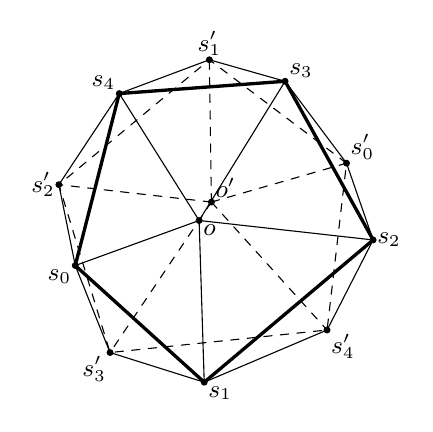
\begin{tikzpicture}[x=0.013cm,y=-0.013cm,line cap=round,line join=round,font=\small]
\coordinate (S0) at (16,201);
\coordinate (S1) at (142,315);
\coordinate (S2) at (307,176);
\coordinate (S3) at (221,21);
\coordinate (S4) at (59,33);
\coordinate (T0) at (281,101);
\coordinate (T1) at (147,0);
\coordinate (T2) at (0,122);
\coordinate (T3) at (50,286);
\coordinate (T4) at (262,264);
\coordinate (O) at (137,157);
\coordinate (Q) at (149,139);
\draw[dashed] (T0)--(T1)--(T2)--(T3)--(T4)--cycle;
\draw[dashed] (Q)--(T0);
\draw[dashed] (Q)--(T1);
\draw[dashed] (Q)--(T2);
\draw[dashed] (Q)--(T3);
\draw[dashed] (Q)--(T4);
\draw (T0)--(S2)--(T4)--(S1)--(T3)--(S0)--(T2)--(S4)--(T1)--(S3)--(T0);
\draw[very thick] (S0)--(S1)--(S2)--(S3)--(S4)--cycle;
\draw (O)--(S0);
\draw (O)--(S1);
\draw (O)--(S2);
\draw (O)--(S3);
\draw (O)--(S4);
\node[below left,inner sep=1.3pt] at (S0) {$s_0$};
\node[below right,inner sep=1.3pt] at (S1) {$s_1$};
\node[right,inner sep=1.3pt] at (S2) {$s_2$};
\node[above right,inner sep=1.3pt] at (S3) {$s_3$};
\node[above left,inner sep=1.3pt] at (S4) {$s_4$};
\node[above right,inner sep=1.3pt] at (T0) {$s'_0$};
\node[above,inner sep=1.3pt] at (T1) {$s'_1$};
\node[left,inner sep=1.3pt] at (T2) {$s'_{2}$};
\node[below left,inner sep=1.3pt] at (T3) {$s'_3$};
\node[below right,inner sep=1.3pt] at (T4) {$s'_4$};
\node[below right,inner sep=1.3pt] at (O) {$o$};
\node[above right,inner sep=1.3pt] at (Q) {$o'$};
\fill (S0) circle[radius=1.25pt];
\fill (S1) circle[radius=1.25pt];
\fill (S2) circle[radius=1.25pt];
\fill (S3) circle[radius=1.25pt];
\fill (S4) circle[radius=1.25pt];
\fill (T0) circle[radius=1.25pt];
\fill (T1) circle[radius=1.25pt];
\fill (T2) circle[radius=1.25pt];
\fill (T3) circle[radius=1.25pt];
\fill (T4) circle[radius=1.25pt];
\fill (Q) circle[radius=1.25pt];
\fill (O) circle[radius=1.25pt];
\end{tikzpicture}}

ou

\figure{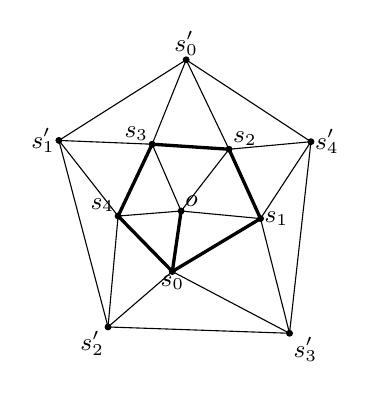
\begin{tikzpicture}[x=0.016cm,y=-0.016cm,line cap=round,line join=round,font=\small]
\coordinate (T0) at (101,0);
\coordinate (T1) at (0,64);
\coordinate (T2) at (39,212);
\coordinate (T3) at (183,217);
\coordinate (T4) at (200,65);
\coordinate (S0) at (90,168);
\coordinate (S1) at (160,126);
\coordinate (S2) at (135,71);
\coordinate (S3) at (74,67);
\coordinate (S4) at (47,124);
\coordinate (O) at (97,120);
\draw (T0)--(T1)--(T2)--(T3)--(T4)--cycle;
\draw (T0)--(S3)--(T1)--(S4)--(T2)--(S0)--(T3)--(S1)--(T4)--(S2)--(T0);
\draw[very thick] (S0)--(S1)--(S2)--(S3)--(S4)--cycle;
\draw[very thick] (O)--(S0);
\draw (O)--(S1);
\draw (O)--(S2);
\draw (O)--(S3);
\draw (O)--(S4);
\node[above,inner sep=1.3pt] at (T0) {$s'_0$};
\node[left,inner sep=1.3pt] at (T1) {$s'_1$};
\node[below left,inner sep=1.3pt] at (T2) {$s'_2$};
\node[below right,inner sep=1.3pt] at (T3) {$s'_3$};
\node[right,inner sep=1.3pt] at (T4) {$s'_4$};
\node[below,inner sep=1.3pt] at (S0) {$s_0$};
\node[right,inner sep=1.3pt] at (S1) {$s_1$};
\node[above right,inner sep=1.3pt] at (S2) {$s_2$};
\node[above left,inner sep=1.3pt] at (S3) {$s_3$};
\node[above left,inner sep=1.3pt] at (S4) {$s_4$};
\node[above right,inner sep=1.3pt] at (O) {$o$};
\fill (T0) circle[radius=1.25pt];
\fill (T1) circle[radius=1.25pt];
\fill (T2) circle[radius=1.25pt];
\fill (T3) circle[radius=1.25pt];
\fill (T4) circle[radius=1.25pt];
\fill (S0) circle[radius=1.25pt];
\fill (S1) circle[radius=1.25pt];
\fill (S2) circle[radius=1.25pt];
\fill (S3) circle[radius=1.25pt];
\fill (S4) circle[radius=1.25pt];
\fill (O) circle[radius=1.25pt];
\end{tikzpicture}}

($\Pi,\Pi'$ deux pent. comb. $\Pi\simeq\Pi'\quad s\longmapsto s'$)

\[
 S=\deleted{\unsure{\{\}}}\inserted{\{o\}\amalg}\Pi\amalg\Pi'\amalg\{o'\}
\]

\diagram{$\begin{array}{llll}
 A=&\left\{\begin{array}{ll}\{o,s\}&s\in\Pi\\\{o',s'\}&s'\in\Pi'\end{array}\right\} &10\\
 &A(\Pi)\quad A(\Pi')&10\\
 &\bigl(\{\underset{\substack{\rotatebox{-90}{$\in$}\\\Pi}}{s},\underset{\substack{\rotatebox{-90}{$\in$}\\\Pi'}}{t}\}\ \unsure{\mid t|\,\not\ni}\,s&10\\
 &\multicolumn{2}{l}{\text{$t$ incident à la face opp. à $s'$}}\\
 &\multicolumn{2}{l}{\text{i.e. }\underset{\substack{\Vert\\\unsure{\delta|d}(t',s)}}{\delta(t,s')}=1}
 \end{array}$}

\textcircled{$A_2$}
\figure{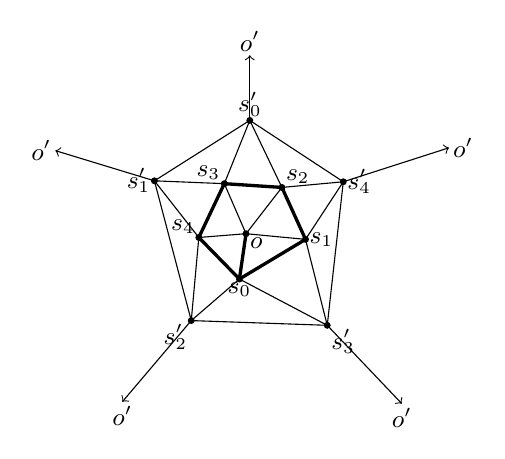
\begin{tikzpicture}[x=0.012cm,y=-0.012cm,line cap=round,line join=round,font=\small]
\coordinate (T0) at (206,69);
\coordinate (T1) at (105,133);
\coordinate (T2) at (144,281);
\coordinate (T3) at (288,286);
\coordinate (T4) at (305,134);
\coordinate (S0) at (195,237);
\coordinate (S1) at (265,195);
\coordinate (S2) at (240,140);
\coordinate (S3) at (179,136);
\coordinate (S4) at (152,193);
\coordinate (O) at (202,189);
\coordinate (E0) at (206,0);
\coordinate (E1) at (0,101);
\coordinate (E2) at (71,367);
\coordinate (E3) at (367,369);
\coordinate (E4) at (417,98);
\draw (T0)--(T1)--(T2)--(T3)--(T4)--cycle;
\draw (T0)--(S3)--(T1)--(S4)--(T2)--(S0)--(T3)--(S1)--(T4)--(S2)--(T0);
\draw[very thick] (S0)--(S1)--(S2)--(S3)--(S4)--cycle;
\draw[very thick] (O)--(S0);
\draw (O)--(S1);
\draw (O)--(S2);
\draw (O)--(S3);
\draw (O)--(S4);
\draw[->] (T0)--(E0);
\draw[->] (T1)--(E1);
\draw[->] (T2)--(E2);
\draw[->] (T3)--(E3);
\draw[->] (T4)--(E4);
\node[above,inner sep=1.3pt] at (T0) {$s'_0$};
\node[left,inner sep=1.3pt] at (T1) {$s'_1$};
\node[below left,inner sep=1.3pt] at (T2) {$s'_2$};
\node[below right,inner sep=1.3pt] at (T3) {$s'_3$};
\node[right,inner sep=1.3pt] at (T4) {$s'_4$};
\node[below,inner sep=1.3pt] at (S0) {$s_0$};
\node[right,inner sep=1.3pt] at (S1) {$s_1$};
\node[above right,inner sep=1.3pt] at (S2) {$s_2$};
\node[above left,inner sep=1.3pt] at (S3) {$s_3$};
\node[above left,inner sep=1.3pt] at (S4) {$s_4$};
\node[below right,inner sep=1.3pt] at (O) {$o$};
\node[above,inner sep=1.3pt] at (E0) {$o'$};
\node[left,inner sep=1.3pt] at (E1) {$o'$};
\node[below,inner sep=1.3pt] at (E2) {$o'$};
\node[below,inner sep=1.3pt] at (E3) {$o'$};
\node[right,inner sep=1.3pt] at (E4) {$o'$};
\fill (T0) circle[radius=1.25pt];
\fill (T1) circle[radius=1.25pt];
\fill (T2) circle[radius=1.25pt];
\fill (T3) circle[radius=1.25pt];
\fill (T4) circle[radius=1.25pt];
\fill (S0) circle[radius=1.25pt];
\fill (S1) circle[radius=1.25pt];
\fill (S2) circle[radius=1.25pt];
\fill (S3) circle[radius=1.25pt];
\fill (S4) circle[radius=1.25pt];
\fill (O) circle[radius=1.25pt];
\end{tikzpicture}}

\noindent\rule{\linewidth}{0.35pt}

\figure{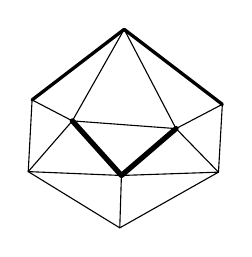
\begin{tikzpicture}[x=0.007cm,y=-0.007cm,line cap=round,line join=round,font=\small]
\coordinate (A) at (174,0);
\coordinate (B) at (0,258);
\coordinate (C) at (345,259);
\coordinate (A1) at (166,360);
\coordinate (B1) at (352,136);
\coordinate (C1) at (7,128);
\coordinate (U) at (169,265);
\coordinate (V) at (268,180);
\coordinate (W) at (80,166);
\coordinate (U1) at (176,121);
\coordinate (V1) at (64,229);
\coordinate (W1) at (282,235);
\draw (A)--(B1)--(C)--(A1)--(B)--(C1)--cycle;
\draw (A)--(W)--(V)--(A);
\draw (B)--(W)--(C1);
\draw (B)--(U)--(C);
\draw (C)--(V)--(B1);
\draw (U)--(A1);
\draw[line width=1.9pt] (W)--(U)--(V);
\draw[very thick] (C1)--(A)--(B1);
\end{tikzpicture}}

\figure{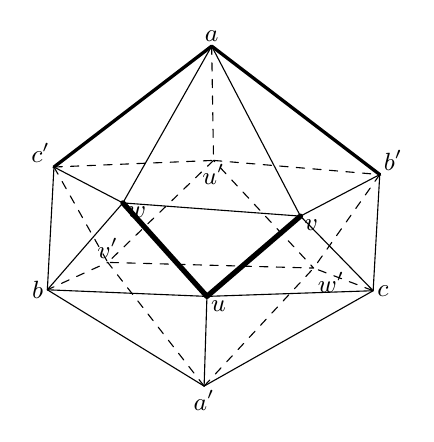
\begin{tikzpicture}[x=0.012cm,y=-0.012cm,line cap=round,line join=round,font=\small]
\coordinate (A) at (174,0);
\coordinate (B) at (0,258);
\coordinate (C) at (345,259);
\coordinate (A1) at (166,360);
\coordinate (B1) at (352,136);
\coordinate (C1) at (7,128);
\coordinate (U) at (169,265);
\coordinate (V) at (268,180);
\coordinate (W) at (80,166);
\coordinate (U1) at (176,121);
\coordinate (V1) at (64,229);
\coordinate (W1) at (282,235);
\draw[dashed] (A)--(U1)--(C1);
\draw[dashed] (U1)--(B1);
\draw[dashed] (U1)--(V1)--(W1)--cycle;
\draw[dashed] (A1)--(V1)--(B);
\draw[dashed] (A1)--(W1)--(C);
\draw[dashed] (C1)--(V1);
\draw[dashed] (B1)--(W1);
\draw (A)--(B1)--(C)--(A1)--(B)--(C1)--cycle;
\draw (A)--(W)--(V)--(A);
\draw (B)--(W)--(C1);
\draw (B)--(U)--(C);
\draw (C)--(V)--(B1);
\draw (U)--(A1);
\draw[line width=1.9pt] (W)--(U)--(V);
\draw[very thick] (C1)--(A)--(B1);
\node[above,inner sep=1.3pt] at (A) {$a$};
\node[left,inner sep=1.3pt] at (B) {$b$};
\node[right,inner sep=1.3pt] at (C) {$c$};
\node[below,inner sep=1.3pt] at (A1) {$a'$};
\node[above right,inner sep=1.3pt] at (B1) {$b'$};
\node[above left,inner sep=1.3pt] at (C1) {$c'$};
\node[below right,inner sep=1.3pt] at (U) {$u$};
\node[below right,inner sep=1.3pt] at (V) {$v$};
\node[below right,inner sep=1.3pt] at (W) {$w$};
\node[below,inner sep=1.3pt] at (U1) {$u'$};
\node[above,inner sep=1.3pt] at (V1) {$v'$};
\node[below right,inner sep=1.3pt] at (W1) {$w'$};
\end{tikzpicture}}

% archive sheet number: 6

\scanpage{8}

(B)

\textcircled{$B_1$}
\figure{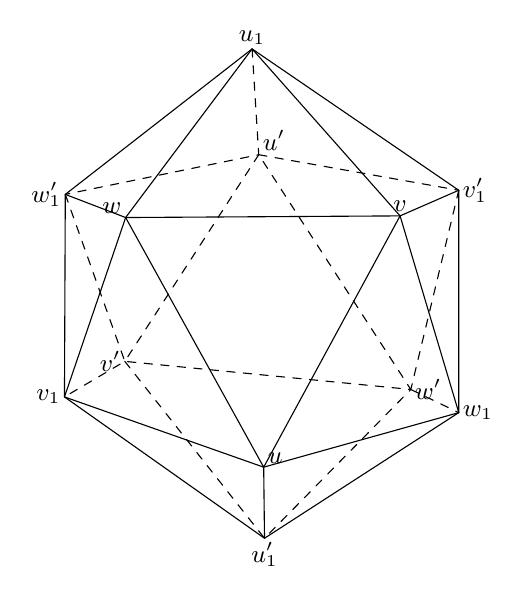
\begin{tikzpicture}[x=0.0105cm,y=-0.0105cm,line cap=round,line join=round,font=\small]
\coordinate (H) at (227,0);
\coordinate (L) at (0,421);
\coordinate (R) at (477,440);
\coordinate (J) at (242,592);
\coordinate (K) at (477,171);
\coordinate (M) at (1,176);
\coordinate (U) at (241,506);
\coordinate (V) at (406,202);
\coordinate (W) at (74,204);
\coordinate (Up) at (235,128);
\coordinate (Vp) at (73,378);
\coordinate (Wp) at (419,412);
\draw[dashed] (H)--(Up)--(M);
\draw[dashed] (Up)--(K);
\draw[dashed] (Up)--(Vp)--(Wp)--cycle;
\draw[dashed] (M)--(Vp)--(L);
\draw[dashed] (Vp)--(J)--(Wp)--(K);
\draw[dashed] (Wp)--(R);
\draw (H)--(M)--(L)--(J)--(R)--(K)--cycle;
\draw (M)--(W)--(V)--(K);
\draw (L)--(W)--(H)--(V)--(R);
\draw (L)--(U)--(R);
\draw (J)--(U);
\draw (W)--(U)--(V);
\node[above,inner sep=1.3pt] at (H) {$u_1$};
\node[left,inner sep=1.3pt] at (L) {$v_1$};
\node[right,inner sep=1.3pt] at (R) {$w_1$};
\node[below,inner sep=1.3pt] at (J) {$u'_1$};
\node[right,inner sep=1.3pt] at (K) {$v'_1$};
\node[left,inner sep=1.3pt] at (M) {$w'_1$};
\node[above right,inner sep=1.3pt] at (U) {$u$};
\node[above,inner sep=1.3pt] at (V) {$v$};
\node[above left,inner sep=1.3pt] at (W) {$w$};
\node[above right,inner sep=1.3pt] at (Up) {$u'$};
\node[left,inner sep=1.3pt] at (Vp) {$v'$};
\node[right,inner sep=1.3pt] at (Wp) {$w'$};
\end{tikzpicture}}

groupe de symétrie $\mathbb Z/2\mathbb Z\times\unsure{\mathfrak S|\mathcal S}_3$ d'ordre $12=120/10$

\uline{NB} $10=20/2$

\figure{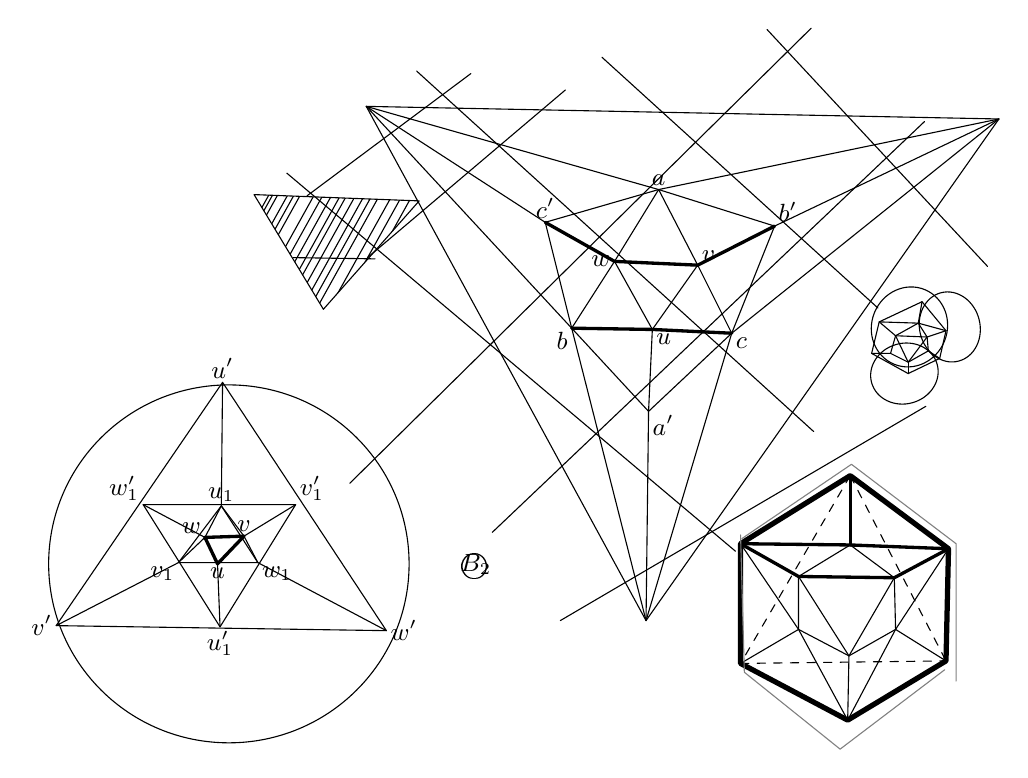
\begin{tikzpicture}[x=0.016cm,y=-0.016cm,line cap=round,line join=round,font=\small]
\coordinate (T) at (246,62);
\coordinate (Q) at (748,72);
\coordinate (Zz) at (468,470);
\coordinate (A) at (478,128);
\coordinate (B) at (409,238);
\coordinate (C) at (536,242);
\coordinate (Ap) at (470,304);
\coordinate (Bp) at (570,157);
\coordinate (Cp) at (388,154);
\coordinate (U) at (473,239);
\coordinate (V) at (509,188);
\coordinate (W) at (443,185);
\coordinate (I) at (157,132);
\coordinate (J) at (288,137);
\coordinate (K) at (212,223);
\coordinate (X) at (188,182);
\coordinate (Y) at (253,183);
\coordinate (H) at (329,36);
\coordinate (Hh) at (199,133);
\coordinate (N) at (404,49);
\coordinate (Nn) at (247,182);
\coordinate (P) at (599,0);
\coordinate (Pp) at (233,361);
\coordinate (Qq) at (689,74);
\coordinate (Qe) at (346,400);
\coordinate (Xx) at (286,34);
\coordinate (Xe) at (601,320);
\coordinate (Yy) at (433,23);
\coordinate (Ye) at (652,222);
\coordinate (Z1) at (564,1);
\coordinate (Z2) at (739,189);
\coordinate (L1) at (183,115);
\coordinate (L2) at (539,415);
\coordinate (Gl) at (400,470);
\coordinate (Gr) at (690,300);
\coordinate (Ht) at (132,281);
\coordinate (Hl) at (0,474);
\coordinate (Hr) at (262,478);
\coordinate (Lt) at (69,378);
\coordinate (Rt) at (190,378);
\coordinate (Bt) at (130,475);
\coordinate (Ut) at (131,379);
\coordinate (Vt) at (97,424);
\coordinate (Wt) at (160,424);
\coordinate (Ui) at (128,425);
\coordinate (Vi) at (149,403);
\coordinate (Wi) at (118,404);
\coordinate (D0) at (630,355);
\coordinate (D1) at (543,409);
\coordinate (D2) at (543,504);
\coordinate (D3) at (628,549);
\coordinate (D4) at (706,502);
\coordinate (D5) at (708,413);
\coordinate (Dt) at (630,410);
\coordinate (F1) at (589,435);
\coordinate (F2) at (665,436);
\coordinate (F3) at (629,498);
\coordinate (F4) at (589,477);
\coordinate (F5) at (666,477);
\coordinate (S0) at (687,217);
\coordinate (S1) at (653,233);
\coordinate (S2) at (647,258);
\coordinate (S3) at (676,274);
\coordinate (S4) at (701,262);
\coordinate (S5) at (706,240);
\coordinate (St) at (684,234);
\coordinate (Si) at (666,244);
\coordinate (Sj) at (691,245);
\coordinate (Sk) at (676,265);
\coordinate (Sl) at (662,258);
\coordinate (Sm) at (692,256);
\coordinate (Badge) at (333,427);
\draw[thin] (T)--(Q)--(Zz)--cycle;
\draw (T)--(Cp);
\draw (T)--(A);
\draw (T)--(B);
\draw (Q)--(A);
\draw (Q)--(Bp);
\draw (Q)--(C);
\draw (Zz)--(Ap);
\draw (Zz)--(B);
\draw (Zz)--(C);
\draw (A)--(Bp)--(C)--(Ap)--(B)--(Cp)--cycle;
\draw[very thick] (Cp)--(W)--(V)--(Bp);
\draw (B)--(W)--(A)--(V)--(C);
\draw[very thick] (B)--(U)--(C);
\draw (Ap)--(U);
\draw (W)--(U)--(V);
\draw[thin] (H)--(Hh);
\draw[thin] (N)--(Nn);
\draw[thin] (P)--(Pp);
\draw[thin] (Qq)--(Qe);
\draw[thin] (Xx)--(Xe);
\draw[thin] (Yy)--(Ye);
\draw[thin] (Z1)--(Z2);
\draw[thin] (L1)--(L2);
\draw[thin] (Gl)--(Gr);
\draw (I)--(J)--(K)--cycle;
\draw[thin] (X)--(Y);
\draw (Ht)--(Hl)--(Hr)--cycle;
\draw (Lt)--(Rt)--(Bt)--cycle;
\draw (Ht)--(Ut);
\draw (Hl)--(Vt);
\draw (Hr)--(Wt);
\draw (Ut)--(Vt)--(Wt)--cycle;
\draw (Bt)--(Ui);
\draw[very thick] (Wi)--(Vi)--(Ui)--cycle;
\draw (Lt)--(Wi)--(Ut)--(Vi)--(Rt);
\draw (Vt)--(Wi);
\draw (Wt)--(Vi);
\draw[line width=1.9pt] (D0)--(D1)--(D2)--(D3)--(D4)--(D5)--cycle;
\draw[very thick] (D1)--(Dt)--(D5);
\draw[very thick] (D0)--(Dt);
\draw[very thick] (D1)--(F1)--(F2)--(D5);
\draw (Dt)--(F1)--(F4)--(D2);
\draw (Dt)--(F2)--(F5)--(D4);
\draw (F1)--(F3)--(F2);
\draw (F4)--(F3)--(F5);
\draw (F3)--(D3);
\draw (D1)--(F4)--(D3)--(F5)--(D5);
\draw[dashed] (D2)--(D4);
\draw[dashed] (D0)--(D2);
\draw[dashed] (D0)--(D4);
\draw (S0)--(S1)--(S2)--(S3)--(S4)--(S5)--cycle;
\draw[thin] (S1)--(St)--(S5);
\draw[thin] (S0)--(St);
\draw[thin] (S1)--(Si)--(Sj)--(S5);
\draw[thin] (St)--(Si)--(Sl)--(S2);
\draw[thin] (St)--(Sj)--(Sm)--(S4);
\draw[thin] (Si)--(Sk)--(Sj);
\draw[thin] (Sl)--(Sk)--(Sm);
\draw[thin] (Sk)--(S3);
\node[above,inner sep=1.3pt] at (A) {$a$};
\node[below left,inner sep=1.3pt] at (B) {$b$};
\node[below right,inner sep=1.3pt] at (C) {$c$};
\node[below right,inner sep=1.3pt] at (Ap) {$a'$};
\node[above right,inner sep=1.3pt] at (Bp) {$b'$};
\node[above,inner sep=1.3pt] at (Cp) {$c'$};
\node[below right,inner sep=1.3pt] at (U) {$u$};
\node[above right,inner sep=1.3pt] at (V) {$v$};
\node[left,inner sep=1.3pt] at (W) {$w$};
\node[above,inner sep=1.3pt] at (Ht) {$u'$};
\node[left,inner sep=1.3pt] at (Hl) {$v'$};
\node[right,inner sep=1.3pt] at (Hr) {$w'$};
\node[above left,inner sep=1.3pt] at (Lt) {$w'_1$};
\node[above right,inner sep=1.3pt] at (Rt) {$v'_1$};
\node[below,inner sep=1.3pt] at (Bt) {$u'_1$};
\node[above,inner sep=1.3pt] at (Ut) {$u_1$};
\node[below left,inner sep=1.3pt] at (Vt) {$v_1$};
\node[below right,inner sep=1.3pt] at (Wt) {$w_1$};
\node[below,inner sep=1.3pt] at (Ui) {$u$};
\node[above,inner sep=1.3pt] at (Vi) {$v$};
\node[above left,inner sep=1.3pt] at (Wi) {$w$};
\node[anchor=center,inner sep=1.3pt] at (Badge) {\textcircled{$B_2$}};
\draw (137,425) ellipse [x radius=143,y radius=142];
\draw[thin] (677,237) ellipse[x radius=30,y radius=32,rotate=-22];
\draw[thin] (709,237) ellipse[x radius=24,y radius=28,rotate=14];
\draw[thin] (673,274) ellipse[x radius=27,y radius=24,rotate=16];
\begin{scope}\clip (I)--(J)--(K)--cycle;
\foreach \t in {152,157,162,167,180,183,187,195,200,205,216,223,230,237,242,249,256,262,268,278,286,294} \draw[thin] (\t,112)--++(-60,108);
\end{scope}
\draw[gray,thin] (543,402)--(546,511)--(622,572)--(705,509);
\draw[gray,thin] (544,405)--(631,346)--(714,409)--(714,518);
\end{tikzpicture}}
% crop-candidate: scan 8

% Left-hand hatched triangle in the preceding TikZ picture.

% Three loops beside the right-hand construction lines.

% Circular projection at lower left of the same picture.

% Heavy hexagon, inner solid and lighter construction strokes at lower right.

% archive sheet number: 7

\scanpage{9}

\figure{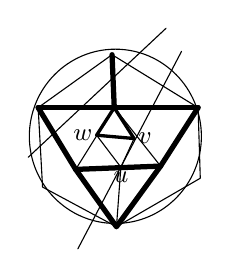
\begin{tikzpicture}[x=0.014cm,y=-0.014cm,line cap=round,line join=round,font=\small]
\coordinate (A) at (76,24);
\coordinate (B) at (9,72);
\coordinate (C) at (154,72);
\coordinate (D) at (80,180);
\coordinate (E) at (13,144);
\coordinate (F) at (156,136);
\coordinate (T) at (78,72);
\coordinate (U) at (43,128);
\coordinate (V) at (120,125);
\coordinate (W) at (62,97);
\coordinate (X) at (96,100);
\coordinate (Y) at (84,126);
\coordinate (L) at (125,0);
\coordinate (R) at (0,117);
\coordinate (J) at (139,21);
\coordinate (K) at (45,200);
\draw (A)--(B)--(E)--(D)--(F)--(C)--cycle;
\draw[line width=1.9pt] (B)--(T)--(C);
\draw[line width=1.9pt] (B)--(U)--(D)--(V)--(C);
\draw[line width=1.9pt] (U)--(V);
\draw[line width=1.9pt] (A)--(T);
\draw[very thick] (T)--(W)--(X)--cycle;
\draw (W)--(Y)--(X);
\draw (T)--(U);
\draw (T)--(V);
\draw (Y)--(D);
\draw[thin] (L)--(R);
\draw[thin] (J)--(K);
\node[left,inner sep=1.3pt] at (W) {$\unsure{w}$};
\node[right,inner sep=1.3pt] at (X) {$v$};
\node[below,inner sep=1.3pt] at (Y) {$u$};
\draw (79,98) ellipse[x radius=78,y radius=79];
\end{tikzpicture}}

\[
 S=T\amalg T_1\amalg T'_1\amalg T'_{\deleted{\unsure{1|2}}}
\]

\diagram{\begin{tikzcd}[ampersand replacement=\&,column sep=small,row sep=large,execute at end picture={\draw (topT.north west) rectangle (topPrime.south east); \path (topT.north) -- node[above] {$t\mapsto t'$} (topPrime.north);}]
t\arrow[d]\& |[alias=topT]| T\arrow[r,"\sim" description]\arrow[d,phantom,"\simeq" description]\& |[alias=topPrime]| T'\arrow[d,phantom,"\simeq" description]\&t'\arrow[d]\\
t_1\&T_1\arrow[r,"\sim","{t_1\mapsto t'_1}"']\&T'_1\&t'_1
\end{tikzcd}}

\deleted{\unsure{triangles}} couple de 2 triangles en corr 1-1

($B_3$)
\figure{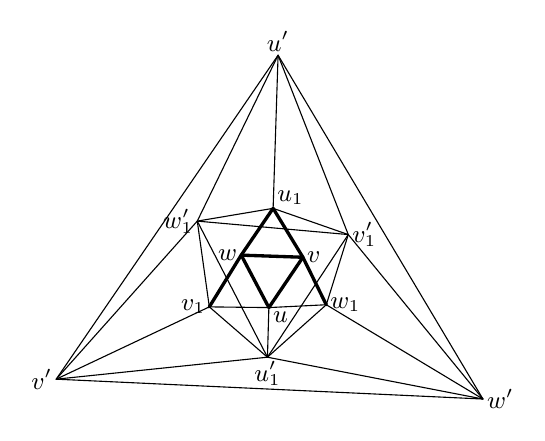
\begin{tikzpicture}[x=0.009cm,y=-0.009cm,line cap=round,line join=round,font=\small]
\coordinate (A) at (313,0);
\coordinate (B) at (0,457);
\coordinate (C) at (602,485);
\coordinate (M) at (199,234);
\coordinate (N) at (412,253);
\coordinate (P) at (298,426);
\coordinate (A1) at (306,216);
\coordinate (B1) at (216,355);
\coordinate (C1) at (381,352);
\coordinate (U) at (300,356);
\coordinate (V) at (348,285);
\coordinate (W) at (261,282);
\draw (A)--(B)--(C)--cycle;
\draw (A)--(M)--(B);
\draw (A)--(N)--(C);
\draw (B)--(P)--(C);
\draw (A)--(A1);
\draw (B)--(B1);
\draw (C)--(C1);
\draw (M)--(N)--(P)--cycle;
\draw (M)--(A1)--(N)--(C1)--(P)--(B1)--cycle;
\draw[very thick] (A1)--(W)--(U)--(V)--cycle;
\draw[very thick] (B1)--(W)--(V)--(C1);
\draw (B1)--(U)--(C1);
\draw (P)--(U);
\node[above,inner sep=1.3pt] at (A) {$u'$};
\node[left,inner sep=1.3pt] at (B) {$v'$};
\node[right,inner sep=1.3pt] at (C) {$w'$};
\node[left,inner sep=1.3pt] at (M) {$w'_1$};
\node[right,inner sep=1.3pt] at (N) {$v'_1$};
\node[below,inner sep=1.3pt] at (P) {$u'_1$};
\node[above right,inner sep=1.3pt] at (A1) {$u_1$};
\node[left,inner sep=1.3pt] at (B1) {$v_1$};
\node[right,inner sep=1.3pt] at (C1) {$w_1$};
\node[below right,inner sep=1.3pt] at (U) {$u$};
\node[right,inner sep=1.3pt] at (V) {$v$};
\node[left,inner sep=1.3pt] at (W) {$w$};
\end{tikzpicture}}

\diagram{$A\ \text{(arêtes)}\quad
\begin{array}{lll}
 \bigl\{\ \mathfrak P_2(T)&\mathfrak P_2(T')&6\\
 \left\{\begin{array}{c}\{\underset{\substack{\rotatebox{-90}{$\in$}\\T}}{t},\underset{\substack{\rotatebox{-90}{$\in$}\\T_1}}{u}\}\\u\ne t_1\end{array}\right.&
 \begin{array}{c}\{\underset{\substack{\rotatebox{-90}{$\in$}\\T'}}{t'},\underset{\substack{\rotatebox{-90}{$\in$}\\T'_1}}{u'}\}\\u'\ne t'_1\end{array}&12\\
 \left\{\begin{array}{c}\{\underset{\substack{\rotatebox{-90}{$\in$}\\T_1}}{\unsure{t|t_1}},\underset{\substack{\rotatebox{-90}{$\in$}\\T'_1}}{u}\}\\u\ne t'\end{array}\right.&&6\\
 \bigl\{\ \{t,t'_1\},\ \{t',t_1\}&&6
\end{array}$}

(C)

($C_1$)
\figure{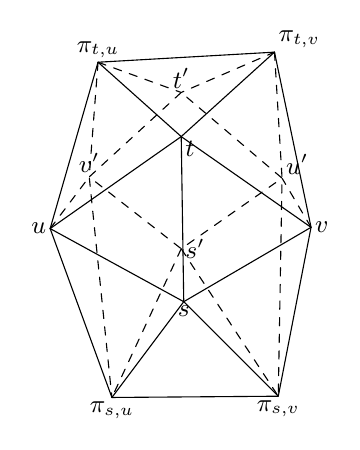
\begin{tikzpicture}[x=0.016cm,y=-0.016cm,line cap=round,line join=round,font=\small]
\coordinate (NW) at (38,8);
\coordinate (NE) at (178,0);
\coordinate (SW) at (49,274);
\coordinate (SE) at (181,273);
\coordinate (L) at (0,140);
\coordinate (R) at (207,139);
\coordinate (T) at (104,67);
\coordinate (S) at (106,198);
\coordinate (Tp) at (104,32);
\coordinate (Sp) at (104,156);
\coordinate (Lp) at (31,99);
\coordinate (Rp) at (184,100);
\draw (NW)--(NE)--(R)--(SE)--(SW)--(L)--cycle;
\draw (NW)--(T)--(NE);
\draw (L)--(T)--(R);
\draw (L)--(S)--(R);
\draw (T)--(S);
\draw (SW)--(S)--(SE);
\draw[dashed] (NW)--(Lp)--(SW);
\draw[dashed] (NE)--(Rp)--(SE);
\draw[dashed] (NW)--(Tp)--(NE);
\draw[dashed] (Tp)--(Lp)--(Sp)--(Rp)--cycle;
\draw[dashed] (Sp)--(SW);
\draw[dashed] (Sp)--(SE);
\draw[dashed] (L)--(Lp);
\draw[dashed] (R)--(Rp);
\node[above,inner sep=1.3pt] at (NW) {$\pi_{t,u}$};
\node[above right,inner sep=1.3pt] at (NE) {$\pi_{t,v}$};
\node[below,inner sep=1.3pt] at (SW) {$\pi_{s,u}$};
\node[below,inner sep=1.3pt] at (SE) {$\pi_{s,v}$};
\node[left,inner sep=1.3pt] at (L) {$u$};
\node[right,inner sep=1.3pt] at (R) {$v$};
\node[below right,inner sep=1.3pt] at (T) {$t$};
\node[below,inner sep=1.3pt] at (S) {$s$};
\node[above,inner sep=1.3pt] at (Tp) {$t'$};
\node[right,inner sep=1.3pt] at (Sp) {$s'$};
\node[above,inner sep=1.3pt] at (Lp) {$v'$};
\node[above right,inner sep=1.3pt] at (Rp) {$u'$};
\end{tikzpicture}}

ou

($C_2$)
\figure{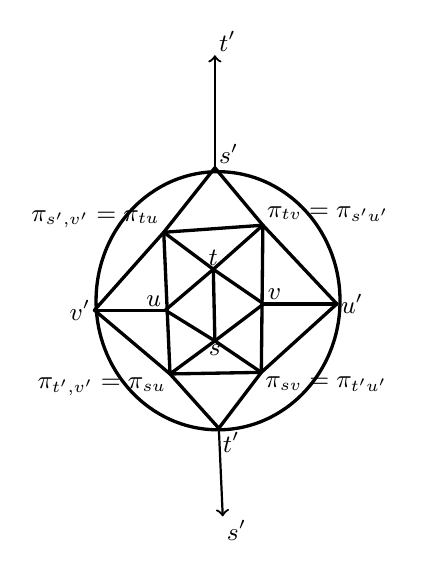
\begin{tikzpicture}[x=0.01cm,y=-0.01cm,line cap=round,line join=round,font=\small]
\coordinate (T) at (153,143);
\coordinate (B) at (158,474);
\coordinate (L) at (0,324);
\coordinate (R) at (308,316);
\coordinate (Nu) at (88,225);
\coordinate (Nv) at (214,216);
\coordinate (Su) at (96,405);
\coordinate (Sv) at (212,403);
\coordinate (U) at (90,324);
\coordinate (V) at (215,316);
\coordinate (Tt) at (151,272);
\coordinate (St) at (153,363);
\coordinate (E) at (153,0);
\coordinate (D) at (163,586);
\draw[very thick] (T)--(Nu)--(L)--(Su)--(B)--(Sv)--(R)--(Nv)--cycle;
\draw[very thick] (Nu)--(Nv)--(Sv)--(Su)--cycle;
\draw[very thick] (U)--(Tt)--(V)--(St)--cycle;
\draw[very thick] (Tt)--(St);
\draw[very thick] (U)--(L);
\draw[very thick] (V)--(R);
\draw[very thick] (Nu)--(Tt)--(Nv);
\draw[very thick] (Su)--(St)--(Sv);
\draw[->,thick] (T)--(E);
\draw[->,thick] (B)--(D);
\node[above right,inner sep=1.3pt] at (T) {$s'$};
\node[below right,inner sep=1.3pt] at (B) {$t'$};
\node[left,inner sep=1.3pt] at (L) {$v'$};
\node[right,inner sep=1.3pt] at (R) {$u'$};
\node[above left,inner sep=1.3pt] at (U) {$u$};
\node[above right,inner sep=1.3pt] at (V) {$v$};
\node[below,inner sep=1.3pt] at (St) {$s$};
\node[above,inner sep=1.3pt] at (Tt) {$t$};
\node[above left,inner sep=1.3pt] at (Nu) {$\pi_{s',v'}=\pi_{tu}$};
\node[above right,inner sep=1.3pt] at (Nv) {$\pi_{tv}=\pi_{s'u'}$};
\node[below left,inner sep=1.3pt] at (Su) {$\pi_{t',v'}=\pi_{su}$};
\node[below right,inner sep=1.3pt] at (Sv) {$\pi_{sv}=\pi_{t'u'}$};
\node[above right,inner sep=1.3pt] at (E) {$t'$};
\node[below right,inner sep=1.3pt] at (D) {$s'$};
\draw[very thick] (157,312) ellipse[x radius=155,y radius=164];
\end{tikzpicture}}

($C_3$)
\figure{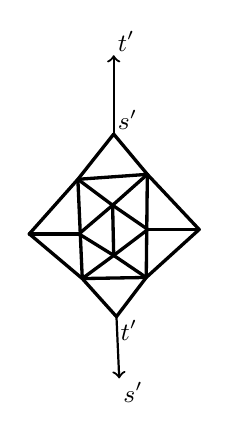
\begin{tikzpicture}[x=0.007cm,y=-0.007cm,line cap=round,line join=round,font=\small]
\coordinate (T) at (153,143);
\coordinate (B) at (158,474);
\coordinate (L) at (0,324);
\coordinate (R) at (308,316);
\coordinate (Nu) at (88,225);
\coordinate (Nv) at (214,216);
\coordinate (Su) at (96,405);
\coordinate (Sv) at (212,403);
\coordinate (U) at (90,324);
\coordinate (V) at (215,316);
\coordinate (Tt) at (151,272);
\coordinate (St) at (153,363);
\coordinate (E) at (153,0);
\coordinate (D) at (163,586);
\draw[very thick] (T)--(Nu)--(L)--(Su)--(B)--(Sv)--(R)--(Nv)--cycle;
\draw[very thick] (Nu)--(Nv)--(Sv)--(Su)--cycle;
\draw[very thick] (U)--(Tt)--(V)--(St)--cycle;
\draw[very thick] (Tt)--(St);
\draw[very thick] (U)--(L);
\draw[very thick] (V)--(R);
\draw[very thick] (Nu)--(Tt)--(Nv);
\draw[very thick] (Su)--(St)--(Sv);
\draw[->,thick] (T)--(E);
\draw[->,thick] (B)--(D);
\draw (T)--(Nv);
\draw (L)--(Nu);
\draw (R)--(Sv);
\draw (B)--(Su);
\node[above right,inner sep=1.3pt] at (T) {$s'$};
\node[below right,inner sep=1.3pt] at (B) {$t'$};
\node[above right,inner sep=1.3pt] at (E) {$t'$};
\node[below right,inner sep=1.3pt] at (D) {$s'$};
\end{tikzpicture}}

\uline{autom.} $\mathbb Z_2\times(\mathbb Z_2\times\mathbb Z_2)$ d'ordre $8=120/15$

\uline{NB} $15=30/2$

\[
 S=\unsure{\sigma|\underline{\sigma}}\amalg\varphi\amalg\sigma'\amalg\varphi'
 \amalg[\sigma\times\varphi\amalg\sigma'\times\varphi'\unsure{\}|/|\sim}]/\mathbb Z/2\mathbb Z
\]

\deleted{$(s,u)\unsure{\sim}(t',v')$ \unsure{si $s\ne t$,}} $\sigma$ opérant par

\[
 \sigma(s,u)=((\varepsilon s)',(\varepsilon u)')
\]

antipodisme \quad $a(s,u)=(\varepsilon s,\varepsilon u)$

\deleted{\unsure{$a$}} $(s,u)\in a\times b$ ou $(s,u)\in(a'\times b')$

\diagram{\begin{tikzpicture}[baseline=(edgeTable.base)]
\node[inner sep=2pt] (edgeTable) {$A:\left|\begin{array}{lll}
 \sigma,\sigma'&\deleted{4}&2\\
 \{\underset{\substack{\rotatebox{-90}{$\in$}\\\sigma}}{s},\underset{\substack{\rotatebox{-90}{$\in$}\\\varphi}}{u}\},\ \{\underset{\substack{\rotatebox{-90}{$\in$}\\\sigma'}}{s'},\underset{\substack{\rotatebox{-90}{$\in$}\\\varphi'}}{u'}\}&&8\\
 \{\pi_{s,u},\pi_{t,v}\}\quad\unsure{u|w}\ 
 \deleted{\unsure{(s,t)}}\ u\ne v &\deleted{\unsure{2|4}}&2\\
 \multicolumn{3}{l}{\hspace{2em}\sigma\quad\varphi\quad\varphi\quad\deleted{\unsure{s,t\ne}}}\\
 \{u,\pi_{s,u}\},\ \{u',\pi_{s',u'}\}&&8\\
 \{s,\pi_{s,u}\},\ \{s',\pi_{s',u'}\}&&8
\end{array}\right.$};
\path (edgeTable.south west) -- coordinate[pos=.56] (ringLeft) coordinate[pos=.84] (ringUpper) (edgeTable.north west);
\path (edgeTable.south east) -- coordinate[pos=.56] (ringRight) coordinate[pos=.84] (ringTopRight) (edgeTable.north east);
\draw (ringLeft) .. controls +(0,-.20) and +(0,-.15) .. (ringRight) .. controls +(.35,0) and +(.35,0) .. (ringTopRight) .. controls +(0,.12) and +(0,.15) .. (ringUpper) .. controls +(-.2,0) and +(-.2,0) .. (ringLeft);
\path (edgeTable.south west) -- coordinate[pos=.43] (leadersEnd) (edgeTable.north west);
\draw[->] (ringLeft) .. controls +(-.38,-.15) and +(-.18,0) .. (leadersEnd);
\end{tikzpicture}}

\[
 \boxed{\{u{},v'\},\ u\ne v\qquad 2}
\]

% archive sheet number: 8

\scanpage{10}

Poly\unsure{è|é}dres réguliers\\
II

\unsure{géométrie|géométries} d'incidences et ens. à opérateurs...

% archive sheet number: 9

\scanpage{11}

\uline{Géométries d'incidences et ensembles à opérateurs}

Soit \inserted{$\Pi=$} $(S,A,F\,;R,R')$ \deleted{\unsure{$P$}} une géométrie d'incidences de dim 2, \deleted{On appelle drapeau} \inserted{$\unsure{\Phi|P|\text{cf.}}$ l'ens ordonné} qu'il définit -- de ``dim. combinatoire'' 2 -- On appelle \uline{drapeau} \inserted{de $\Pi$} une partie tot. ordonnée non vide de $\Pi$ -- si son cardinal est $l$, on dit que le drapeau est de \uline{longueur} $l-1$. Le maximum des longueurs des drapeaux est 2 -- les drapeaux de longueur 2 sont appelés \uline{repères}, leur ens se note $\operatorname{Rep}(\Pi)$

\[
 \operatorname{Rep}(\Pi)\unsure{:|=}\{(\underset{\deleted{\unsure{0}}}{s},a,f)\in S\times A\times F\mid s<a<f\}
\]

Il y a des drapeaux des types suivants

\diagram{$\left.\begin{array}{ccc}0&1&2\\S&A&F\end{array}\right\}
 \begin{array}{l}\text{drapeaux minimaux \inserted{(de long. 0)}}\\\text{ou ``facettes''}\end{array}$}

\diagram{$\left.\begin{array}{ccc}
 (0,1)&(1,2)&(0,2)\\
 R\subset S\times A)&R'\subset A\times F&R''\subset S\times F
 \end{array}\right\}\ \text{drapeaux de long. 1}$}

\diagram{$\left.\begin{array}{c}(0,1,2)\\\operatorname{R\acute ep}\subset S\times A\times F\end{array}\right\}\ 
 \begin{array}{l}\text{repères, ou drapeaux}\\\text{maximaux}\end{array}$}

Il y a des applications naturelles ``d'oubli'' (partiel) entre ces ens. de drapeaux, en particulier

% archive sheet number: 10

\scanpage{12}

\diagram{\begin{tikzcd}[ampersand replacement=\&,row sep=small]
\&\deleted{\operatorname{Rep}}\arrow[dl]\arrow[dr]\&{}\\
\deleted{R\subsetS\times A}\&{}\&\deleted{R'\subset}
\end{tikzcd}}

[ En fait, on part de

\diagram{\begin{tikzcd}[ampersand replacement=\&,column sep=small,row sep=small]
\&R\arrow[dl,"2"']\arrow[dr,"2"]\&{}\&R'\arrow[dl,dash,"2"']\arrow[dr,"\unsure{2}"]\&{}\\
S\&{}\&A\&{}\&F
\end{tikzcd}}

et on construit au-dessus de ceux-ci $\deleted{\unsure{\operatorname{Rep}}}E=\ R\times_A R'$, d'où

\diagram{\begin{tikzcd}[ampersand replacement=\&,column sep=small,row sep=small]
\&\operatorname{Rep}\arrow[dl,"{(\sigma_0)}"']\arrow[d,"{(\sigma_1)}"]\arrow[dr,"{(\sigma_2)}"]\&{}\\
\operatorname{Drap}_{12}=R'\arrow[d,phantom,"\rotatebox{-90}{$\subset$}" description]\&
R''=\operatorname{Drap}_{02}\arrow[d,phantom,"\rotatebox{-90}{$\subset$}" description]\&
R=\deleted{\unsure{R}}\operatorname{Drap}_{01}\arrow[d,phantom,"\rotatebox{-90}{$\subset$}" description]\\
A\timesF\& S\times F\&S\times A
\end{tikzcd}}

\diagram{\begin{tikzcd}[ampersand replacement=\&,column sep=small,row sep=small]
{}\&{}\&E=\operatorname{Rep}\arrow[dl,"2"']\arrow[dr,"2"]\&{}\&{}\\
{}\&R\arrow[dl,"2"']\arrow[dr,"2"]\&{}\&R'\arrow[dl,"2"']\arrow[dr,"2"]\&{}\\
S\&{}\&A\&{}\&F
\end{tikzcd}}

Ces trois applications sont de degré 2 \inserted{(axiomes 1), 2))} -- d'où des involutions sans p\textsuperscript{ts} \unsure{fixes|fixe} dans Rep notées $\sigma_0,\sigma_1,\sigma_2$ qui sont caractérisées par le fait de \unsure{inverser|invarier|conserver} les fibres des applic$^{\mathrm{tions}}$ précédentes (NB $\sigma_i$ change la facette \unsure{composante} de dim $i$ d'un repère $r=(s,a,f)$ et \deleted{\unsure{le}} \unsure{conserve|laisse} les deux autres). On voit que $\sigma_0$ et $\sigma_2$ \deleted{\unsure{On trouve ainsi deux}} commutent

\[
 \sigma_0\sigma_{\unsure{2|1}}(s,a,f)=\sigma_2\sigma_0(s,a,f)=(s',a,f')
\]

où $s'$ est l'unique sommet $\ne s$ incident à $a$

$f'$ \rule{2.4cm}{0.35pt} face $\ne f$ \rule{1.5cm}{0.35pt} $a$

On voit que $\sigma_0,\sigma_1,\sigma_2$ et $\sigma_0\sigma_2$ opèrent sur Rep. sans pt fixe.

Soit

\[
 \unsure{G|\mathcal G|\mathfrak G|\mathfrak S}_2=
 \left\{\sigma_0,\sigma_1,\sigma_2\ \middle|\
 \begin{aligned}
 \sigma_0^2=\sigma_1^2=\sigma_2^2&=1\\
 \sigma_0\sigma_2&=\sigma_2\sigma_0
 \end{aligned}\right\}
\]

% archive sheet number: 11

\scanpage{13}

Donc on a un foncteur

\diagram{\begin{tikzcd}[ampersand replacement=\&,column sep=large]
{\begin{array}{c}\text{Géom. d'incidences}\\\text{(avec iso)}\end{array}}
\arrow[r]\&
{\begin{array}{l}\unsure{G|\mathcal G|\mathfrak G|\mathfrak S}_2\text{-ens. où $\sigma_0,\sigma_1,\sigma_2$}\\
 \text{et $\sigma_0\sigma_2$ opèrent ss pts}\\ \text{fixes (avec iso)}\end{array}}
\end{tikzcd}}

On va voir que \inserted{\uline{Thm}} ce foncteur est \uline{pleinement fidèle} -- donc qu'on peut réconstruire $(S,A,F,R,R')$ à partir de $E=\operatorname{Rep}$ en \deleted{tant} que $G_2$-ens. Notons qu'on a

\[
\begin{aligned}
 E/(\sigma_1,\sigma_2)&\longrightarrow S=\Phi_0\\
 E/(\sigma_0,\sigma_2)&\longrightarrow A=\Phi_1\\
 E/(\sigma_0,\sigma_1)&\longrightarrow F=\Phi_2
\end{aligned}
\]

\deleted{qui sont des applications \uline{surjectives}.}

Il est clair que l'application médiane est un iso [$\sigma_0,\sigma_2$ engendrent un ss-gpe de $G_2$ $\simeq\mathbb Z_2\times\mathbb Z_2$, qui opère librement sur $E$ \deleted{\unsure{par hyp.},} le quotient est $\xrightarrow{\sim} A$]. Or les axiomes 3) et 3$'$) (pas encore utilisés) expriment respectivement \deleted{\unsure{que sont surjectives}} que la dernière et la première flèches sont \deleted{\unsure{aussi}} \uline{bijectives}. Celà permet d'exprimer $S,A,F$ à partir de $R$.

% archive sheet number: 12

\scanpage{14}

Quant : $R,R'$, ce sont respectivement les images de $E=\operatorname{Rep}$ dans $S\times A$ et $A\times F$ ....

\uline{Corollaire} \deleted{Les autom. de} gpe $\operatorname{Aut}(\Pi)$ s'identifie à $\operatorname{Aut}_{\unsure{G|\mathcal G|\mathfrak G|\mathfrak S}_2\text{-ens}}(\operatorname{Rep}(\Pi))$.

\uline{Corollaire} Conditions équivalentes

a) Deux sommets de $\Pi$ sont \inserted{tjrs} reliés par une chaine d'\unsure{arê\textsuperscript{tes}|aires|arêtes}

a$'$) Deux faces de $\Pi$ sont \inserted{tjrs} reliées par une chaine d'arêtes

\[
 \text{b)}\quad\Pi\simeq\Pi'\amalg\Pi''\ \Longrightarrow\ \Pi'=\varnothing\ \text{ou}\ \Pi''=\varnothing.
\]

c) \deleted{\unsure{le}} $G_2$ opère \uline{transitivement} dans $E$\inserted{$=\operatorname{Rep}(\Pi)$}. (i.e. -- si $\Pi\ne\varnothing$ i.e. $E\ne\varnothing$ \deleted{\unsure{\}}} -- $E$ est un \uline{espace homogène} sous $G_2$)

\deleted{Corollaire} \uline{Déf} On dit alors que $\Pi$ est connexe.

\uline{Corollaire} Si $\Pi$ est connexe, $\operatorname{Aut}\Pi$ opère librement dans $\operatorname{Rep}(\Pi)$, i.e. si $g\in\operatorname{Aut}(\Pi)$, $r\in\operatorname{Rep}(\Pi)$, alors

\[
 g.r=r\quad\Longrightarrow\quad g=\mathrm{id}
\]

En effet, un autom d'un espace homogène qui fixe un pt, \deleted{fixe l'espace homogène.} \inserted{est l'identité}.

% archive sheet number: 13

\scanpage{15}

\uline{Corollaire} (Si $\Pi$ fini :) $\operatorname{Card}\operatorname{Aut}(\Pi)\mid\operatorname{Card}\operatorname{Rep}(\Pi)$

\uline{Re-corollaire} Conditions équivalentes pour $\Pi$ connexe (\deleted{\unsure{fixé|soit}} \inserted{le} $r\in\inserted{E=}\operatorname{Rep}(\Pi)$ fixé)

a) $\inserted{G=}\operatorname{Aut}(\Pi)$ est transitif sur $\operatorname{Rep}(\Pi)$

b) Le stabilisateur de \deleted{un} $r$ est un ss-groupe \uline{distingué} de $\unsure{G|\mathcal G|\mathfrak G|\mathfrak S}_2$

c) (Si $\Pi$ est fini) $\operatorname{Card}\operatorname{Aut}(\Pi)=\operatorname{Card}\operatorname{Rep}(\Pi)$

d) $\forall g\in G_2,\ \exists\,\bar g\in G$ tel que $g.r=\bar g.r$

d$'$) $\forall\,0\leq i\leq2,\ \exists\,\bar\sigma_i\in G$ tel que $\sigma_i r=\bar\sigma_i r$, (i.e.

\margin{$\unsure{\sigma_i|\bar\sigma_i}r\ne r$ et $\sigma_{\unsure{j|i}}r$ coïncide avec $r$ en dim $\ne\unsure{j|i}$}

\uline{Déf} On dit alors que la géom. d'incidences est régulière (on parle aussi de polyèdre combinatoire régulier ...)

\uline{Cor.} Soient $(\Pi_0,r_0)$ \deleted{\unsure{polygone}}polyèdre régulier avec repère, $\Pi$ \deleted{\unsure{polygone}}polyèdre régulier isom. à $\Pi_0$. Alors

\[
 \begin{aligned}
 \operatorname{Isom}(\Pi_0,\Pi)&\xrightarrow{\sim}\operatorname{Rep}\unsure{\Pi)|(\Pi)}\\
 \varphi&\longmapsto\varphi(r_0)
 \end{aligned}
\]

En particulier : Un couple $(\Pi_0,r_0)$, pour un type d'isomorphie \uline{donné} de $\Pi_0$, est défini à isom$^{\mathrm{ie}}$ unique près ...

\uline{Corollaire}

\diagram{\begin{tikzcd}[ampersand replacement=\&,row sep=0.2em,execute at end picture={\foreach \c in {1,2} {\draw (\tikzcdmatrixname-1-\c.north west) -- (\tikzcdmatrixname-3-\c.south east); \draw (\tikzcdmatrixname-1-\c.north east) -- (\tikzcdmatrixname-3-\c.south west);}}]
\deleted{E/\sigma_0}\arrow[r,"\sim"]\&\deleted{\operatorname{Drap}_{1\,2}(\Pi)}\\
\deleted{E/\sigma_1}\arrow[r,"\sim"]\&\deleted{\operatorname{Drap}_{0,2}(\Pi)}\\
\deleted{E/\sigma_2}\arrow[r,"\sim"]\&\deleted{\operatorname{Drap}_{0,1}(\Pi)}
\end{tikzcd}}

\deleted{Soit \unsure{$T$}} \inserted{Avec les notations} de d) ci-dessus, $g\mapsto\bar g$ est un épi de $G_2$ sur $G$. En particulier

% archive sheet number: 14

\scanpage{16}

\deleted{[ Soit $\Pi=(S,\ldots)$ une géométrie d'incidences, $R^+\subset E=\operatorname{Rep},\ R^-=E\smallsetminus R^+$. Conditions équivalentes}

\deleted{a) $\sigma_i R^+=R^-\quad(i=0,1,2)$}

\deleted{b) $R^+\xrightarrow{\sim}\unsure{{}'}\,\unsure{\underline{\omega}|\underline{\Phi}|\Psi}_{i}=\prod_{j\ne i}\Phi_j\quad(i=0,1,2)$ où $\Phi_0=S,\ \Phi_1=A,\ \Phi_2=F$}

\deleted{On dit alors que $R^+$ est une \uline{orientation}, et les $r\in R^+$ sont les \uline{repères directs} pour cette \deleted{\unsure{orientation}}, \inserted{(ou compatibles avec)}, les $r\in{\unsure{\Pi|R}}^-$ les \uline{repères inverses} ]}

\deleted{Soit $\Pi$ polyèdre régulier connexe de type $(p,q)$. Groupe des autom. d'un polyèdre régulier $\Pi$ qui fixent un sommet : C' \deleted{est} le groupe diédral $D_p$ (\inserted{plus précis} groupe des autom du polygône}

\margin{\deleted{($p=\text{ordre}(\sigma_1\sigma_2)_E,\ q=\text{ordre}(\sigma_0\sigma_1)_E$}}

\figure{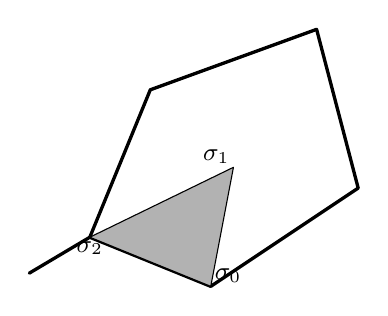
\begin{tikzpicture}[x=0.024cm,y=-0.024cm,line cap=round,line join=round,font=\small]
\coordinate (A) at (32,110);
\coordinate (B) at (64,32);
\coordinate (C) at (152,0);
\coordinate (D) at (174,84);
\coordinate (E) at (96,136);
\coordinate (O) at (108,73);
\coordinate (X) at (0,129);
\draw[very thick] (A)--(B)--(C)--(D);
\draw[very thick] (D)--(E);
\draw[very thick] (E)--(A);
\draw[very thick] (A)--(X);
\draw[fill=black!30] (A)--(O)--(E)--cycle;
\node[above left,inner sep=1.3pt] at (O) {$\sigma_{\unsure{1}}$};
\node[above right,inner sep=1.3pt] at (E) {$\sigma_0$};
\node[below,inner sep=1.3pt] at (A) {$\sigma_2$};
\end{tikzpicture}}

les $\bar\sigma_i$ engendrent $G$.

\margin{(Exer)}
% slanted

\uline{Proposition} Soit $\Pi$ \deleted{\unsure{polygone}}\unsure{polyèdre} \inserted{comb.} régulier connexe, $E=\operatorname{Rep}(\Pi)$, $G=\operatorname{Aut}(\Pi)$, $\Phi=$ ens des facettes de $\Pi$. --

a) Soit $p=\text{ordre}\,(\sigma_{\unsure{1}}\sigma_2)_E$, $q=\inserted{\text{ordre}}\,(\sigma_0\sigma_1)_E$. Alors par tt sommet de $\deleted{\unsure{E}}\Pi$ passent exact$^{\mathrm{t}}$ $p$ arêtes, \deleted{par} \inserted{sur} tte face il y a exact$^{\mathrm{t}}$ $q$ arêtes

(\uline{NB} $3\leq p,q\leq+\infty$).

b) Soit $s\in S(\Pi)$. Alors le hom du stabilisateur $G_s$ de \inserted{$s$ ds} $G$, dans $\operatorname{Aut}(\Phi_{\geq s})$ [ où $\Phi_{\geq s}$ est le polygône combinatoire à $p$ côtés

% archive sheet number: 15

\scanpage{17}

formé des facettes incidentes à $s$) est un iso. En particulier $G_s\simeq\mathbb D_p$

b$'$) Soit $f\in F(\Pi)$. Alors $G_f\to\operatorname{Aut}(\Phi_{\leq f})$ (où $\Phi_{\leq f}$ est le polygône combinatoire à $q$ côtés des facettes incidentes à $f$) est un iso. En particulier, $G_f\simeq D_q$.

\unsure{c|b}) Soit $a\in A(\Pi)$. \deleted{Alors} Soit $\sigma$ \inserted{($\varphi$)} l'ens des sommets (faces) incidents à $a$. -- donc $\sigma,\varphi$ sont des ens. de card. 2.

Considérons

\[
 G_a\longrightarrow\unsure{\mathfrak S|\mathcal S}_{\sigma}\times\mathfrak S_{\varphi}=\mathbb Z/2\mathbb Z\times\mathbb Z/2\mathbb Z
\]

C'est un \uline{iso}.

\deleted{\uline{Exer} \uline{Proposition} Soit $\Pi$ polyèdre \inserted{comb.} régulier connexe fini, Pour tt $s\in S$,}

% archive sheet number: 16

